\subsubsection{\stid{1.07} Exascale MPI} \label{subsubsect:mpich}
\paragraph{Overview}

MPI has been the de facto standard programming model for HPC from the
mid 90's till today, a period where supercomputing performance
increased by six orders of magnitude.  The vast majority of DOE's
parallel scientific applications running on the largest HPC systems
use MPI.  These application codes represent billions of dollars of
investment.  Therefore, MPI must evolve to run as efficiently as
possible on Exascale systems.  Our group at Argonne developed a
high-performance, production-quality MPI implementation, called MPICH.
The focus areas of the Exascale MPI / MPICH project are: (1)
continuous improvement of the performance and capabilities of the
MPICH software to meet the demands of ECP and other broader DOE
applications, (2) coordinate vendor and supercomputing center
interactions to ensure efficient solutions to applications, and (3) be
involved in the MPI forum and standardization efforts to ensure
continuity of the work beyond this project.

MPICH team is  involved in the formation of the MPI Forum and have been
deeply involved in defining the MPI standard since 1992. MPICH has helped
prototype and define the majority of the features in the MPI standard.
As such, MPICH has been one of the most influential pieces of software in accelerating
the adoption of the MPI standard by the HPC community. MPICH has been adopted by leading
vendors into their own derivative implementations. Examples include Intel (for Intel MPI),
Cray (for Cray MPI), IBM (for IBM PE MPI), Mellanox (for MLNX-MPI), Microsoft (for MS-MPI),
and Ohio State University (for MVAPICH). MPICH and its derivatives are exclusively used in
8 of the top 10 supercomputers in the world today.
MPICH is the recipient of a number of awards including an R\&D 100 award.

\paragraph{Key  Challenges}

While we believe MPI is a viable programming model at Exascale, both
the MPI standard and MPI implementations have to address the
challenges posed by the increased scale, performance characteristics
and evolving architectural features expected in Exascale systems, as
well as the capabilities and requirements of applications targeted at
these systems.  The key challenges are:

\begin{enumerate}

\item Interoperability with intranode programming models having a high
  thread count \cite{Hybrid1, Hybrid2, FT2} (such as OpenMP,
  OpenACC and emerging asynchronous task models);

\item Scalability and performance over complex architectures
  \cite{Perf1, Perf2, FT2, Perf4} (including high core counts,
  processor heterogeneity and heterogeneous memory);

\item Software overheads that are exacerbated by lightweight cores and
  low-latency networks;

\item Enhanced functionality (extensions to the MPI standard) based on
  experience with applications and high-level libraries/frameworks
  targeted at Exascale; and

\item Topics that become more significant as we move to the next
  generation of HPC architectures: memory usage, power, and
  resilience.

\end{enumerate}


\paragraph{Solution Strategy}

The Exascale MPI project has the following primary technical thrusts:
(1) \textbf{Performance and Scalability} (2) \textbf{Heterogeneity}
(3) \textbf{Topology Awareness} (4) \textbf{Fault Tolerance} and (5)
\textbf{MPI+X Hybrid Programming}.

Our solution strategy started by addressing performance and
scalability aspects in MPICH related to network address management
\cite{memscal}.  Apart from this, we also looked at communication
strategies which allow the MPI library to be as lightweight as
possible \cite{ch41, ch42}.  Other solutions include
investigation and evaluation of communication relaxation hints,
investigation of optimizations to memory scalability in MPICH and
improvements to MPI RMA operations.

Exascale MPI heterogeneity efforts \cite{Hetero1, Hetero2, Hetero3}
started with the survey on heterogeneous memory architectures on
upcoming DOE machines and how MPICH can take advantage of them
\cite{hexe}.  The other efforts include the investigation of
utilizing heterogeneous memory inside the MPI implementation and
evaluation of applications.

Exascale MPI topology awareness efforts \cite{Topo1,Topo2} originated
with the investigation and evaluation of hints based on topology
awareness and optimizations to virtual topology functionality in MPICH
\cite{topo-io,topo-io2}.  The ongoing efforts include investigation of
topology-aware collectives and neighborhood collectives in MPICH
\cite{coll} and evaluation of the selected ECP applications.

Exascale MPI fault tolerance efforts \cite{FT1, FT2} started with
support for handling noncatastrophic errors in MPI.  The second effort
included defining the scope of errors in MPI, a prerequisite for
user-level failure mitigation (ULFM).  Other efforts that we are
looking at in this direction are standardizing ULFM in MPI and
evaluating application suitability for fault tolerance.

Exascale MPI+X hybrid programming developed firstly with effort in
improving interoperation of MPICH with threads \cite{interthread}.
Secondly, we included support for interaction of MPICH with user-level
thread (ULT) libraries \cite{ULT}, primarily targeting Argobots and
the BOLT runtime and the work-queue data transfer model for
multithreaded MPI communication.  Other issues that are being looked
at include the investigation and evaluation on interaction between MPI
and OpenMP and the study and evaluation of MPI endpoints.


\paragraph{Recent Progress}

Figure~\ref{fig:sep18} provides the details of the milestones completed in FY18Q3 and FY18Q4.
In the first milestone completed in June 2018, a communicator info hint is proposed to expose
communication progress characteristics to the user to provide a more efficient way of ensuring
MPI progress that results in better application  performance.
In the second milestone completed in June 2018, a study report was submitted on efforts needed to
achieve interoperability between MPI and task and to enable direct transfer of data from
GPU memory to NIC with MPI calls.
In the third milestone completed in June 2018, three categories of applications are investigated: 1)
stencil computation applications; 2)cosmology applications;  3)dynamic  execution  environment  applications.
While these applications currently do
not benefit from ULFM, we think it is still important for us to provide ULFM in the Exascale
MPI library and explore on a broader range of applications.
In the fourth milestone completed in June 2018, a list of recommendations that will be
helpful to users wishing to exploit memory heterogeneity \cite{hetero4} in their MPI codes.

\begin{figure}[htb]
  \centering
  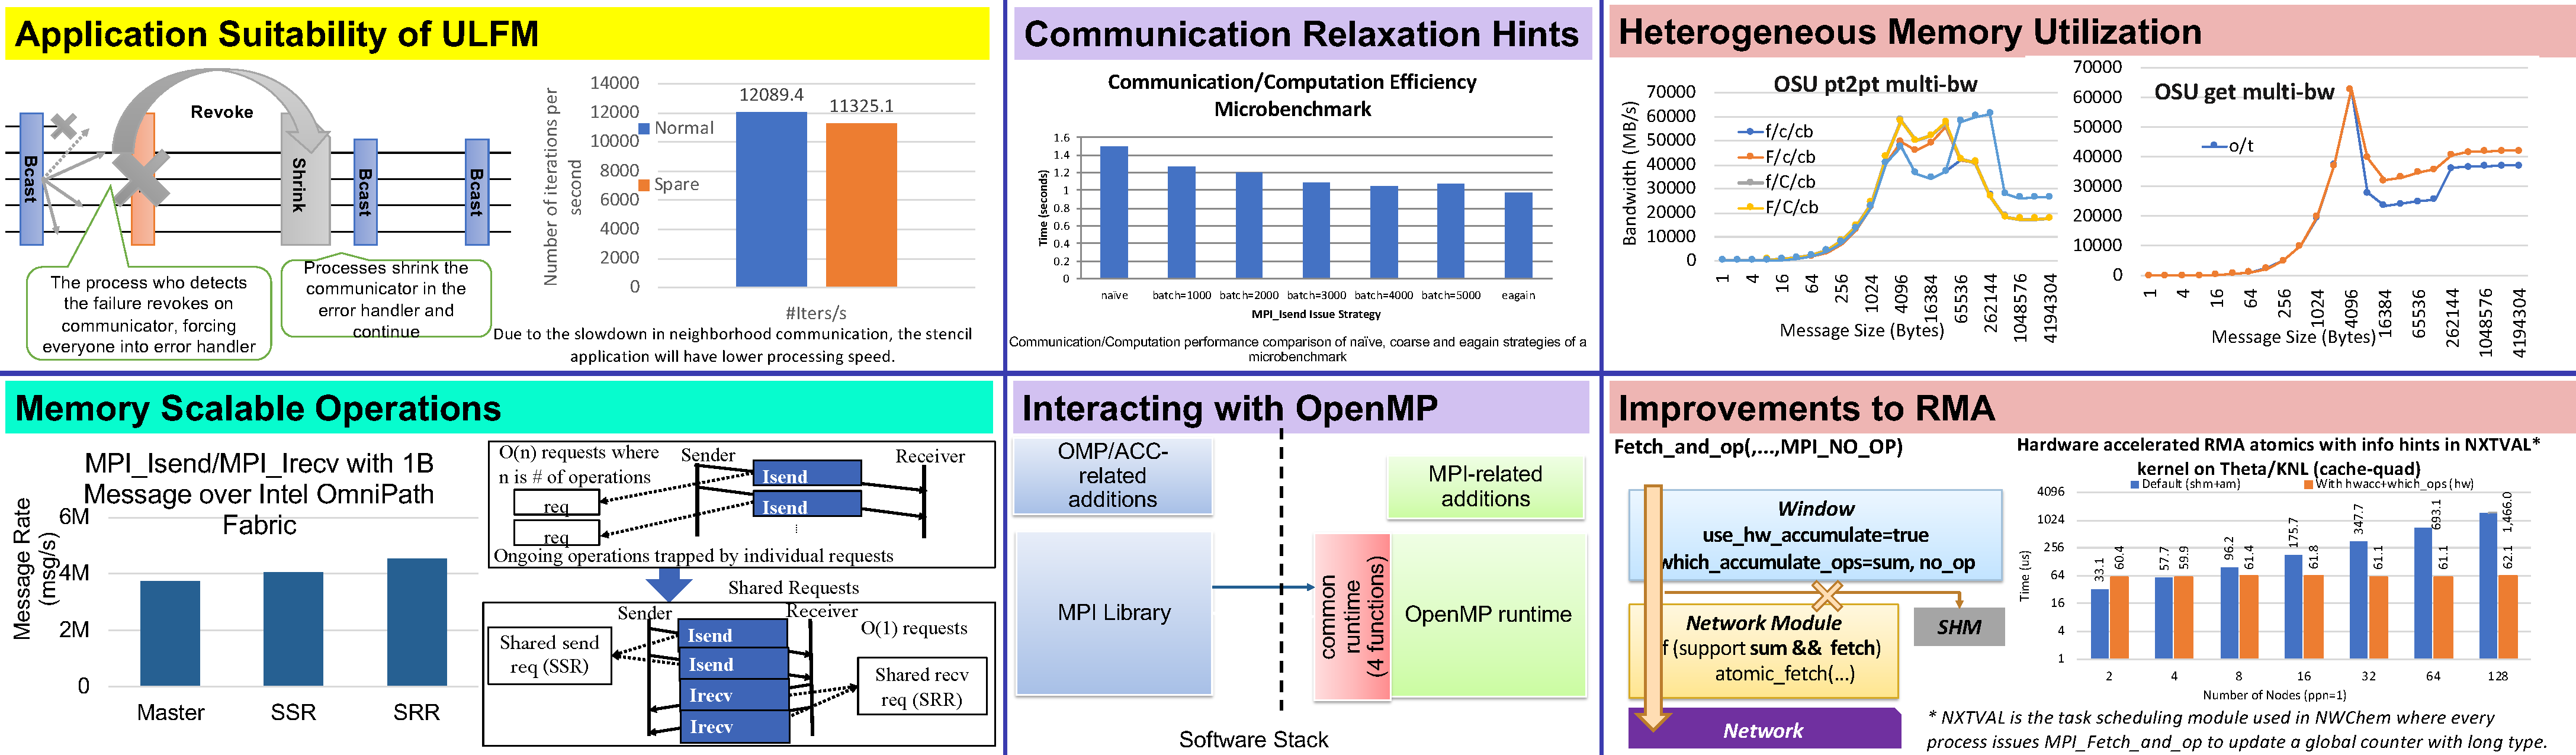
\includegraphics[width=6in]{projects/2.3.1-PMR/2.3.1.07-Exascale-MPI/MPICH-recent-milestones.pdf}
  \caption{\label{fig:sep18}MPICH milestones
    completed in June 2018 and Septmeber 2018}
\end{figure}

In the first milestone completed in September 2018, lightweight send and receive requests
for communication are instroduced. In this
way, we are able to only use constant number of requests to track many operations which
significantly reduce the memory scalability
of MPI. Furthermore, by sharing the preallocated requests, we also avoid the costs
of request allocation and initialization within each operation and achieved even higher message rate.
In the second milestone completed in September 2018, introduced MPI info, "disable\_shm\_accumulate",
to only use network-based atomics for MPI accumulates in specific windows and
"which\_accumulate\_ops", to limit the need of atomic support at runtime.

\paragraph{Next Steps}
Exascale MPI ongoing efforts include ECP application performance evaluation of utilizing
heterogeneous memory inside the MPI implementation, analysis of the performance evaluation
of the implementation of virtual topology functionality, standardization of ULFM
in MPI and finally, investigate and evaluate the implementation of MPI-4 ULFM proposal in MPICH,
to investigate a study of the benefit potential of the MPI endpoints approach and evaluate
it with selected ECP applications and to investigate
topology-aware collectives and neighborhood collectives in MPICH and evaluate the selected ECP applications.
